\documentclass{article}
\usepackage[utf8]{inputenc}
\usepackage{amsmath}
\usepackage[spanish]{babel}
\usepackage{graphicx}
\usepackage{float}


\newcommand\tab[1][1cm]{\hspace*{#1}}
\begin{document}



\section*{Problema B}
Nombre: Juan Sebastian Vargas\\
 Codigo: 201215310\\
Fecha: 20/05/16

\section{Algoritmo Soluci\'on}
La primera parte es la lectura de datos con el formato descrito en el enunciado, un numero, y en una nueva línea,(System.in) se encuentran las pesas.

Para este algoritmo se investigó sobre soluciones posibles y se encontró que tiene cierta similitud con el problema de partición y se utilizo para solucionar este, consta de un método que me dice si un conjunto dado se puede dividir en dos y que la suma de ellos sea igual, notese que si se puede dividir en partes iguales, y de esta manera X seria descubrible. Primero se calcula si la suma del conjunto es par, de caso contrario no se podría dividir, y luego recursivamente se busca un subconjunto que su cumpla esto. 


La idea central es añadir los elementos e ir comprobando si es probable medir x. Con alguna fracción del conjunto inicial. 
Se encontró otra implementación y era usando programación dinámica, la cual puede llegar a ser mucho mas rápida que la que se escogio, pero lo negativo de esta es que implementando programación dinámica la complejidad temporal dependería de la suma de todos los elementos, la cual puede llegar a ser muy grande. Y si el numero de pesas crece, también lo haría la suma

\section{Complejidades}

 Para este paso tenemos una Complejidad Temporal de  $O(2^2)$, pero logramos una Espacial de $O(0)$

\begin{figure}[h]

 \scalebox{0.65}{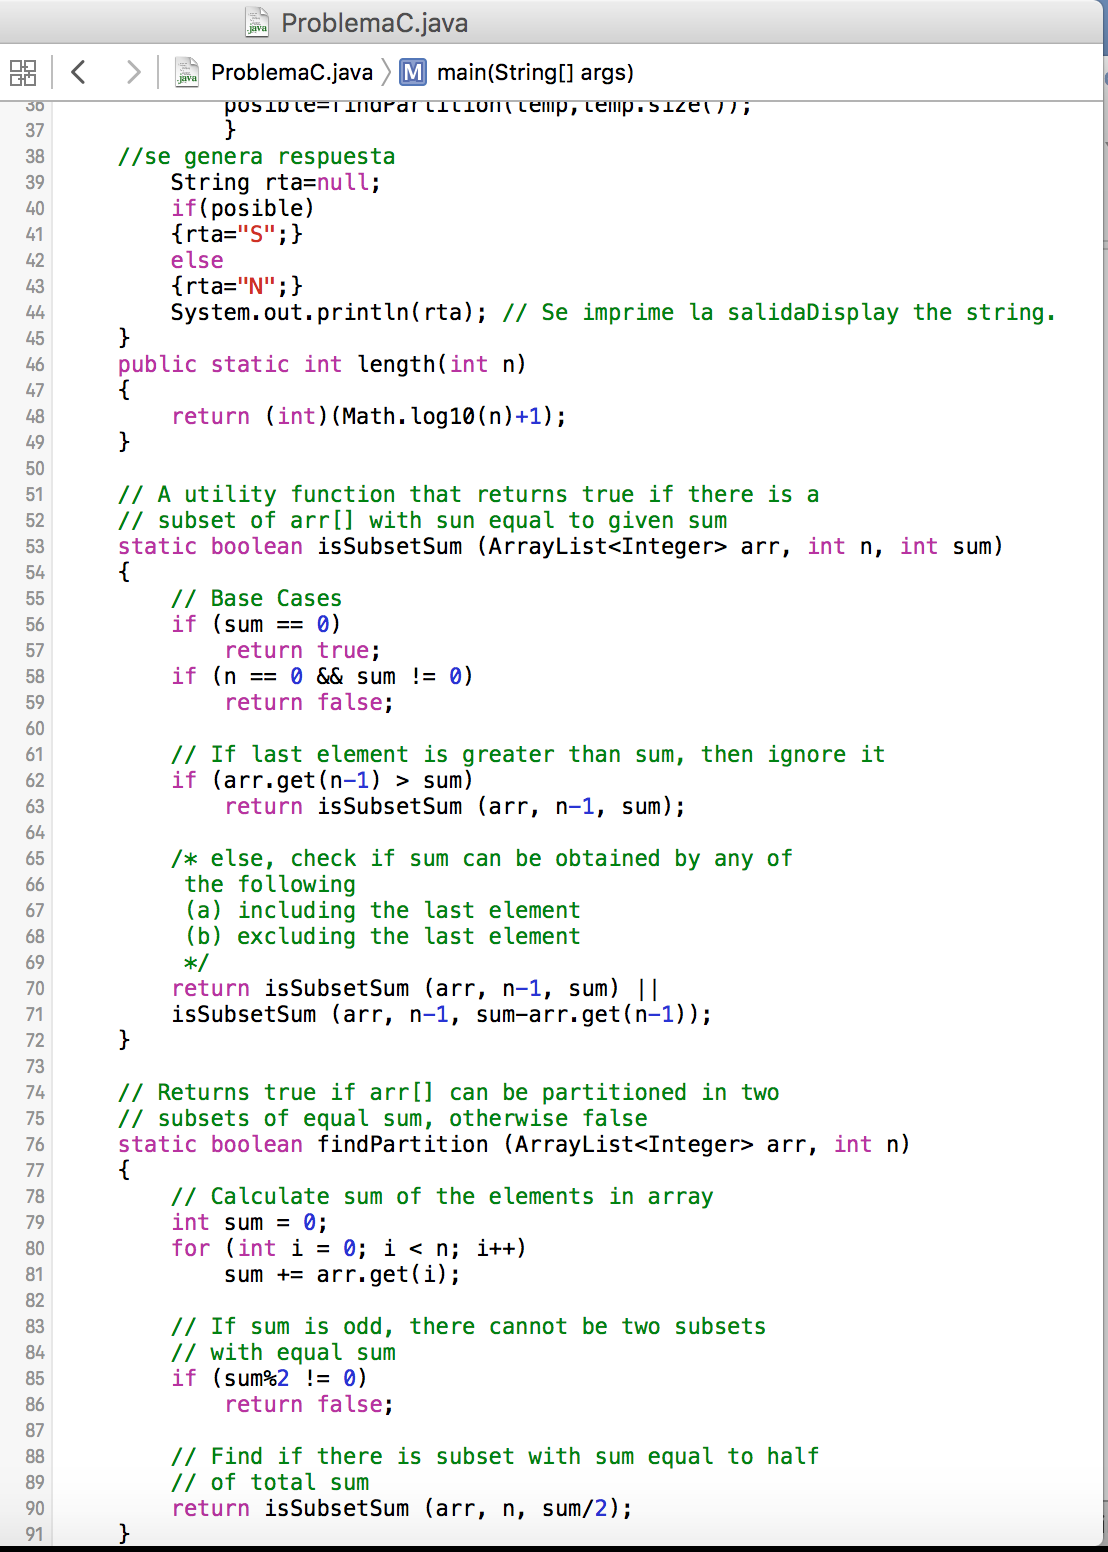
\includegraphics{ProblemaC.png}}
 \caption{Algoritmo}
 \label{Al}
\end{figure}


\end{document}